\subsection{Experimental Setup}
\label{sec:setup}

\subsubsection{System used}

Experiments are performed on a system featuring an AMD EPYC-7742 processor with $64$ cores, operating at a frequency of $2.25$ GHz. Each core is equipped with a $4$ MB L1 cache, a $32$ MB L2 cache, and shares a $256$ MB L3 cache. The server is set up with $512$ GB of DDR4 system memory and runs on Ubuntu $20.04$.


\subsubsection{Configuration}

We utilize 32-bit integers for vertex IDs and 64-bit floating-point numbers for vertex ranks. Affected vertices are represented using an 8-bit integer vector. The rank computation employs OpenMP's \textit{dynamic schedule} with a chunk size of $2048$, facilitating dynamic workload balancing among threads. We use a damping factor of $\alpha = 0.85$ \cite{rank-langville06}, with an iteration tolerance of $\tau = 10^{-10}$ using the $L_\infty$-norm \cite{rank-dubey22, rank-plimpton11}. The maximum number of iterations (\texttt{MAX\_ITERATIONS}) is limited to $500$ \cite{nvgraph}. All experiments are conducted with $64$ threads to match the number of cores available on the system, unless specified otherwise. Compilation is carried out using GCC $9.4$ and OpenMP $5.0$.


\subsubsection{Dataset}

We use the largest five temporal networks from the Stanford Large Network Dataset Collection \cite{snapnets}, as detailed in Table \ref{tab:dataset}. The number of vertices in these graphs range from $X$ million to $X$ million, with temporal edge counts spanning from $X$ million to $X$ billion, and static edge counts spanning from $X$ million to $X$ billion. For the experiment in Section $X$, we use four classes of static graphs (as batch update are randomly generated, with uniform probability for selection of any vertex as the endpoint of an edge to be inserted or deleted), sourced from the \textit{SuiteSparse Matrix Collection} \cite{suite19}, as detailed in Table \ref{tab:dataset}. The number of vertices in these graphs range from $3.07$ million to $214$ million, with edge counts spanning from $37.4$ million to $1.98$ billion. To address the impact of dead ends (vertices lacking out-links), a global teleport rank computation is needed in each iteration. We mitigate this overhead by adding self-loops to all vertices in the graph \cite{rank-andersen07, rank-langville06}.

\begin{table}[hbtp]
  \centering
  \caption{List of 5 real-world dynamic graphs\ignore{, i.e., temporal networks}, obtained from the Stanford Large Network Dataset Collection \cite{snapnets}. Here, $|V|$ is the number of vertices, $|E_T|$ the number of temporal edges\ignore{(includes duplicate edges)}, and $|E|$ the number of static edges (with no duplicates).\ignore{, and $\Gamma_G$ is the Gini coefficient of PageRank distribution. In the table, B refers to a billion, M refers to a million and K refers a thousand.}}
  \label{tab:dataset}
  \begin{tabular}{|c||c|c|c|c|}
    \toprule
    \textbf{Graph} &
    \textbf{\textbf{$|V|$}} &
    \textbf{\textbf{$|E_T|$}} &
    \textbf{\textbf{$|E|$}} \\
    \midrule
    sx-mathoverflow & 24.8K & 507K & 240K \\ \hline
    sx-askubuntu & 159K & 964K & 597K \\ \hline
    sx-superuser & 194K & 1.44M & 925K \\ \hline
    wiki-talk-temporal & 1.14M & 7.83M & 3.31M \\ \hline
    sx-stackoverflow & 2.60M & 63.4M & 36.2M \\ \hline
  \bottomrule
  \end{tabular}
\end{table}



\subsubsection{Batch Generation}
\label{sec:batch-generation}

For each base (static) graph from the dataset, we generate a random batch update, consisting of purely edge insertions, purely edge deletions, or an $80\% : 20\%$ mix of edge insertions and deletions to mimic realistic batch updates. The set of edges for insertion is prepared by selecting vertex pairs with equal probability. To construct the set of edge deletions, we delete each existing edge with a uniform probability. For simplicity, we ensure that no new vertices are added to or removed from the graph. The batch size is measured as a fraction of edges in the original graph, and is varied from $10^{-7}$ to $0.1$ (i.e., $10^{-7}|E|$ to $0.1|E|$), with multiple batches generated for each size (for averaging). Along with each batch update, self-loops are added to all vertices.


\subsubsection{Measurement}
\label{sec:measurement}

We measure the time taken by each approach on the updated graph entirely, including any preprocessing costs and convergence detection time, while excluding time dedicated to memory allocation and deallocation. The mean time for a specific method at a given batch size is calculated as the geometric mean across various input graphs. Consequently, the average speedup is determined as the ratio of these mean times. Additionally, we gauge the error/accuracy of a given approach by assessing the $L1$-norm \cite{ohsaka2015efficient} of the ranks in comparison to ranks obtained from a reference Static PageRank run on the updated graph with an extremely low iteration tolerance of $\tau = 10^{-100}$ (limited to $500$ iterations).

\begin{figure*}[!hbt]
  \centering
  \subfigure[]{
    \label{fig:temporal-all--runtime}
    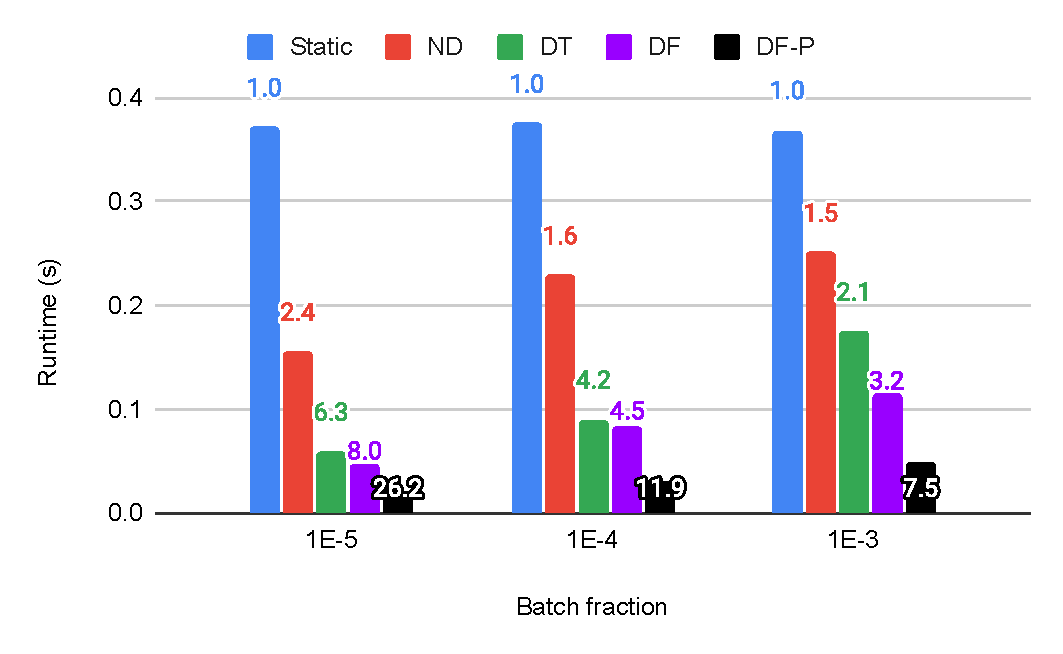
\includegraphics[width=0.48\linewidth]{out/temporal-all-runtime.pdf}
  }
  \subfigure{
    \label{fig:temporal-all--error}
    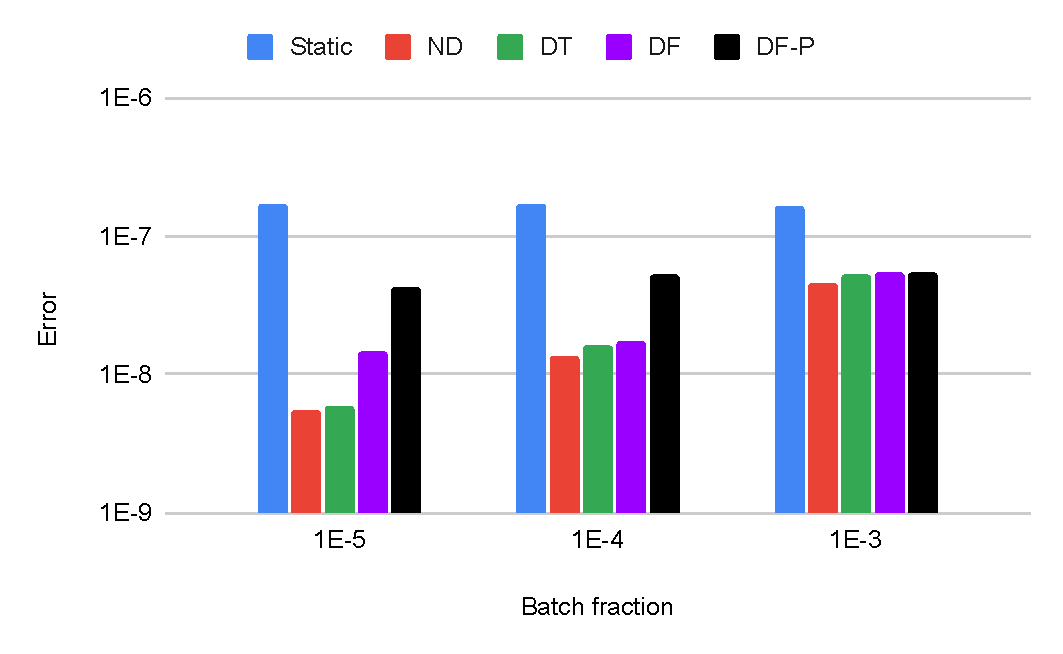
\includegraphics[width=0.48\linewidth]{out/temporal-all-error.pdf}
  } \\[-4ex]
  \caption{Overall Runtime and Error in ranks obtained with \textit{Static}, \textit{Naive-dynamic (ND)}, \textit{Dynamic Traversal (DT)}, and our improved \textit{Dynamic Frontier (DF)} PageRank on real world dynamic graphs, with batch updates of size $10^{-5}|E|$ to $10^{-3}|E|$. In (a), the speedup of each approach with respect to Static PageRank is labeled.}
  \label{fig:temporal-all}
\end{figure*}

\begin{figure*}[!hbt]
  \centering
  \subfigure{
    \label{fig:temporal-batch5--runtime}
    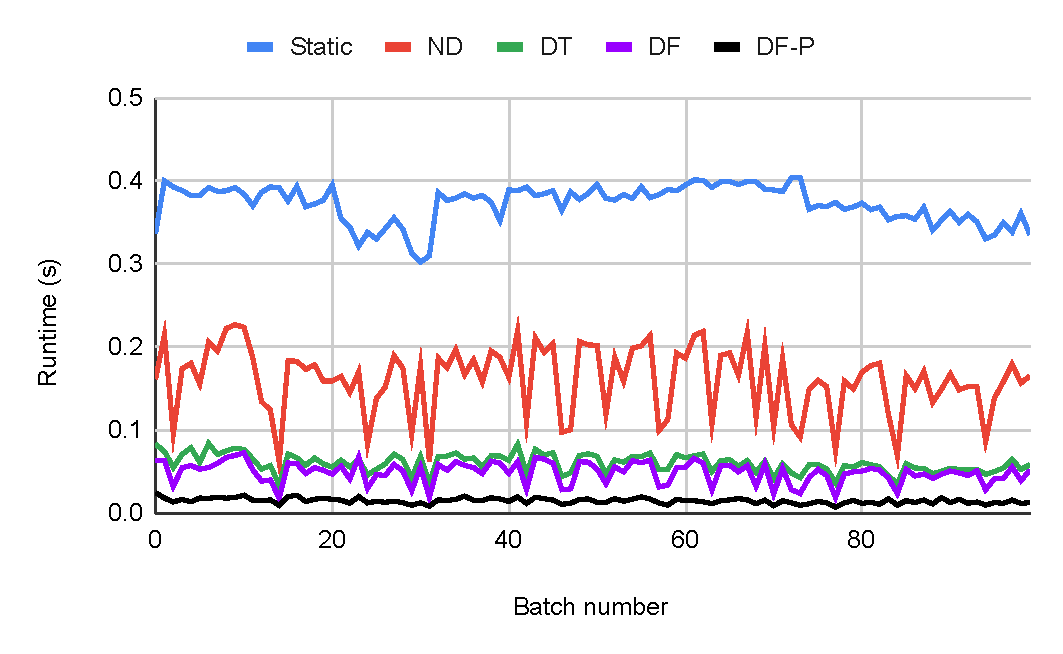
\includegraphics[width=0.48\linewidth]{out/temporal-batch5-runtime.pdf}
  }
  \subfigure{
    \label{fig:temporal-batch5--error}
    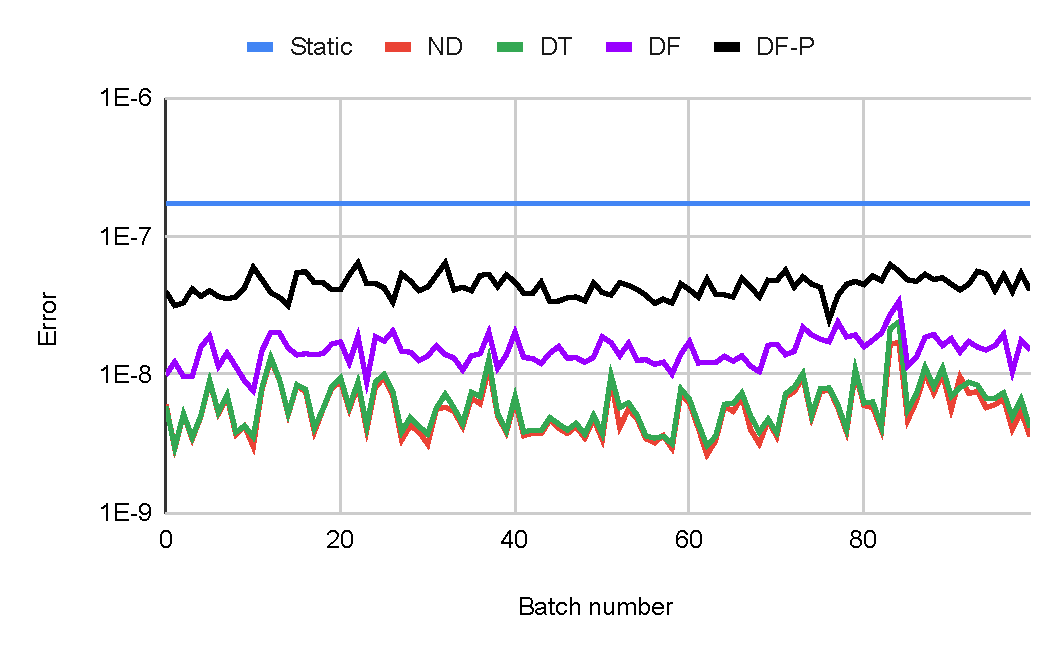
\includegraphics[width=0.48\linewidth]{out/temporal-batch5-error.pdf}
  } \\[-2ex]
  \caption{Average Relative runtime with asynchronous implementations of \textit{Static}, \textit{Naive-dynamic}, \textit{Dynamic Traversal}, and \textit{Dynamic Frontier} approach compared to their respective synchronous implementations, on batch updates of size $10^{-7}|E|$ to $0.1|E|$ (right), and overall (left). The results indicate that asynchronous implementations are faster than synchronous ones, especially for smaller batch sizes. This is due to a somewhat faster convergence and the absence of copy overhead (for \textit{Dynamic Traversal} and \textit{Dynamic Frontier} approaches).}
  \label{fig:temporal-batch5}
\end{figure*}

\begin{figure*}[!hbt]
  \centering
  \subfigure{
    \label{fig:temporal-batch4--runtime}
    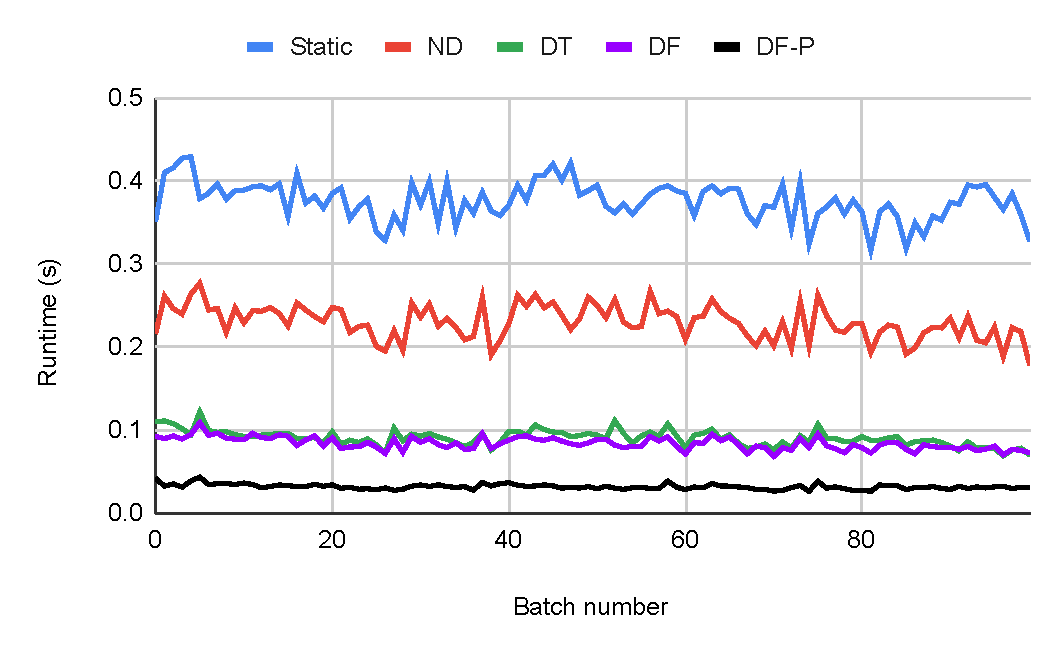
\includegraphics[width=0.48\linewidth]{out/temporal-batch4-runtime.pdf}
  }
  \subfigure{
    \label{fig:temporal-batch4--error}
    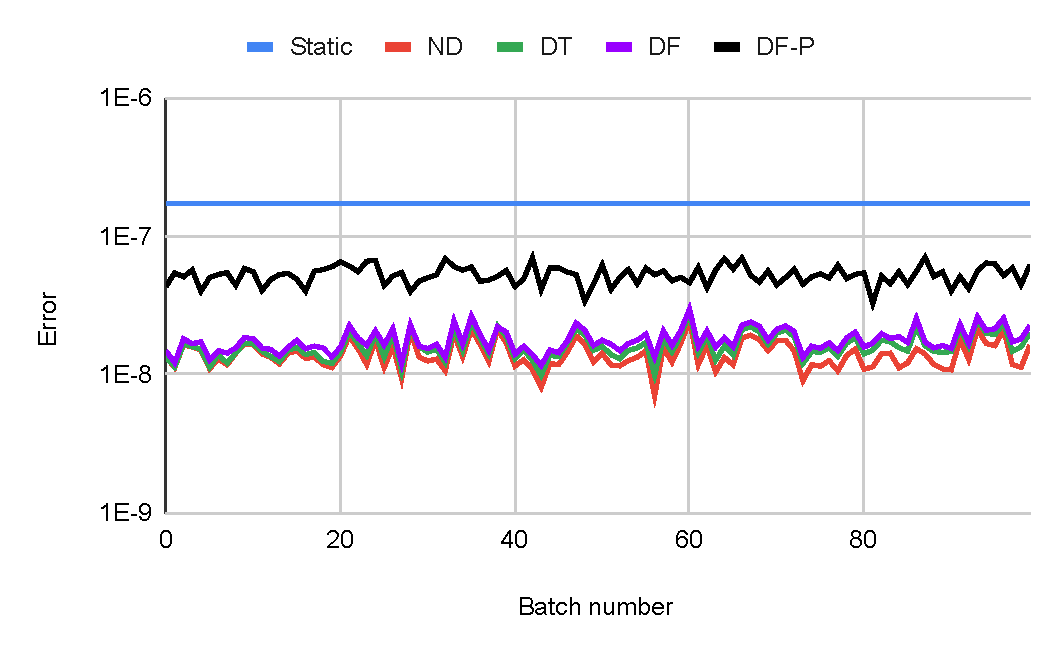
\includegraphics[width=0.48\linewidth]{out/temporal-batch4-error.pdf}
  } \\[-2ex]
  \caption{Average Relative runtime with asynchronous implementations of \textit{Static}, \textit{Naive-dynamic}, \textit{Dynamic Traversal}, and \textit{Dynamic Frontier} approach compared to their respective synchronous implementations, on batch updates of size $10^{-7}|E|$ to $0.1|E|$ (right), and overall (left). The results indicate that asynchronous implementations are faster than synchronous ones, especially for smaller batch sizes. This is due to a somewhat faster convergence and the absence of copy overhead (for \textit{Dynamic Traversal} and \textit{Dynamic Frontier} approaches).}
  \label{fig:temporal-batch4}
\end{figure*}

\begin{figure*}[!hbt]
  \centering
  \subfigure{
    \label{fig:temporal-batch3--runtime}
    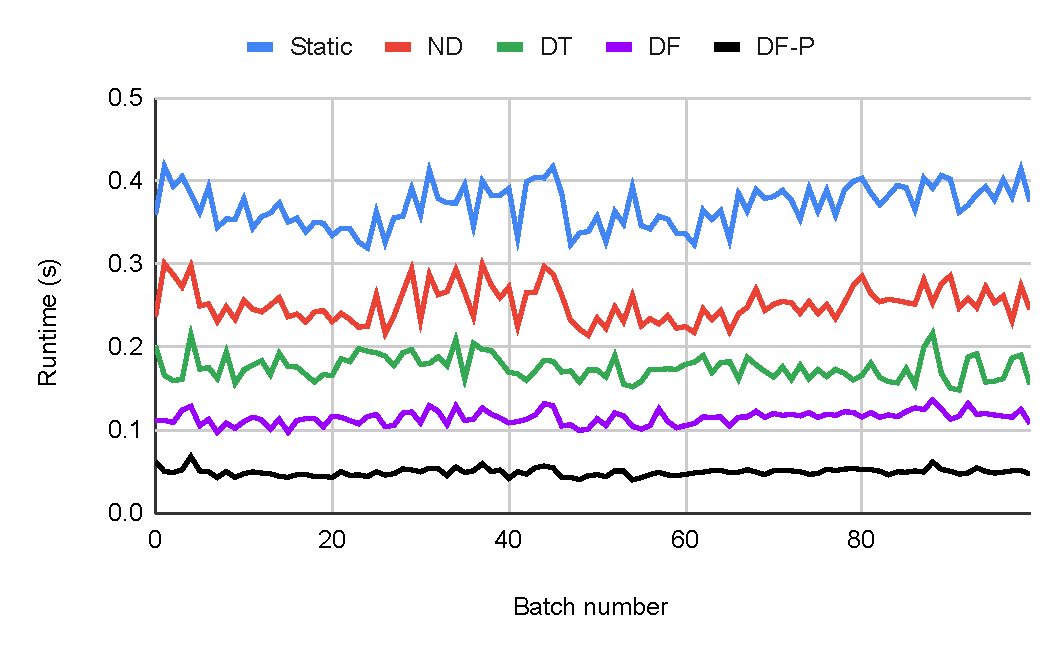
\includegraphics[width=0.48\linewidth]{out/temporal-batch3-runtime.pdf}
  }
  \subfigure{
    \label{fig:temporal-batch3--error}
    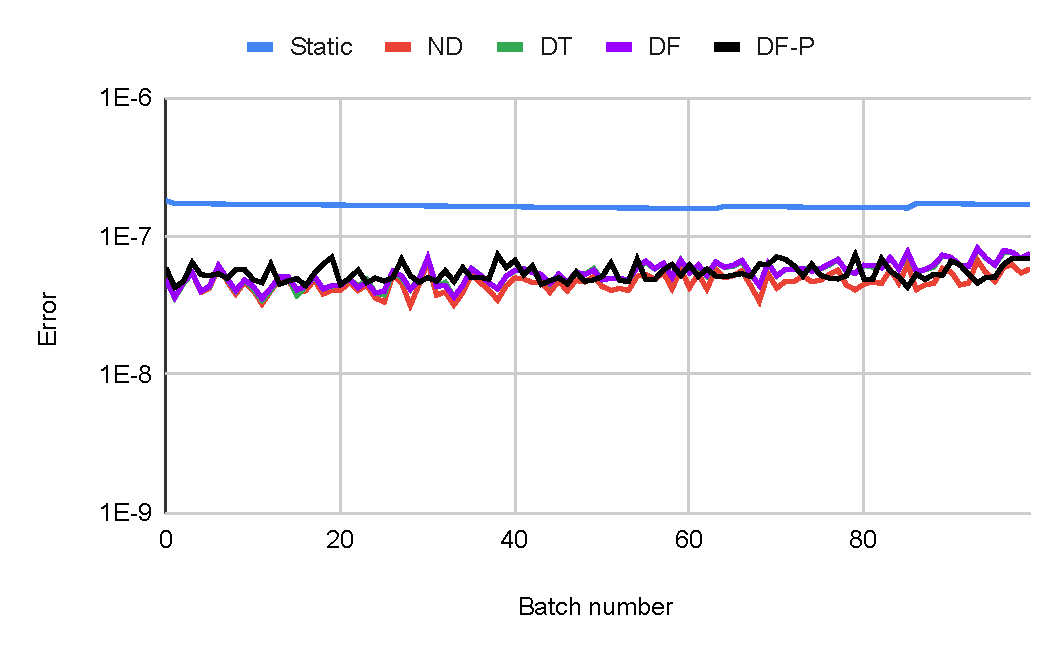
\includegraphics[width=0.48\linewidth]{out/temporal-batch3-error.pdf}
  } \\[-2ex]
  \caption{Average Relative runtime with asynchronous implementations of \textit{Static}, \textit{Naive-dynamic}, \textit{Dynamic Traversal}, and \textit{Dynamic Frontier} approach compared to their respective synchronous implementations, on batch updates of size $10^{-7}|E|$ to $0.1|E|$ (right), and overall (left). The results indicate that asynchronous implementations are faster than synchronous ones, especially for smaller batch sizes. This is due to a somewhat faster convergence and the absence of copy overhead (for \textit{Dynamic Traversal} and \textit{Dynamic Frontier} approaches).}
  \label{fig:temporal-batch3}
\end{figure*}

\begin{figure*}[!hbt]
  \centering
  \subfigure{
    \label{fig:temporal-large--runtime}
    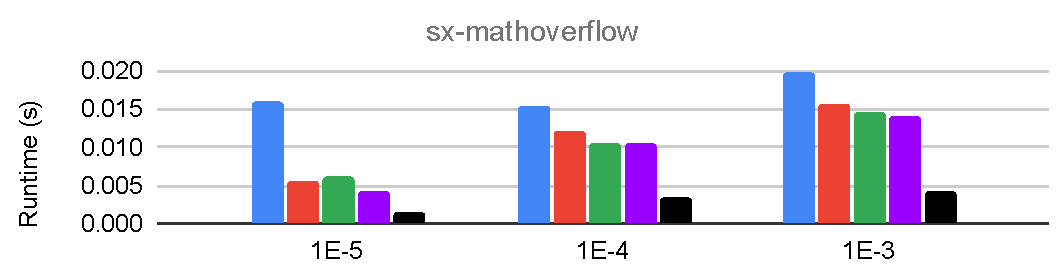
\includegraphics[width=0.48\linewidth]{out/temporal-large-runtime-sx-mathoverflow.pdf}
  }
  \subfigure{
    \label{fig:temporal-large--error}
    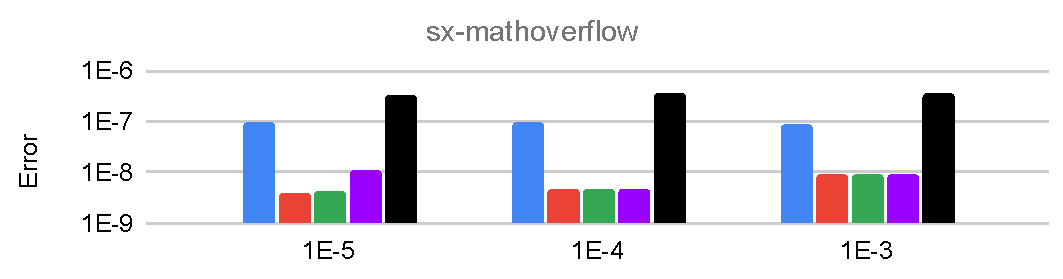
\includegraphics[width=0.48\linewidth]{out/temporal-large-error-sx-mathoverflow.pdf}
  }
  \subfigure{
    \label{fig:temporal-large--runtime}
    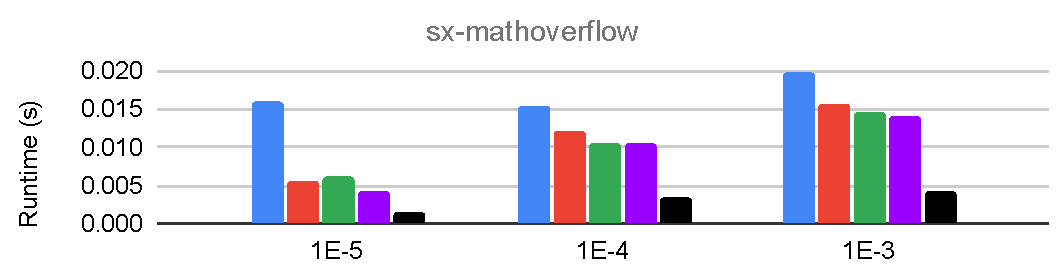
\includegraphics[width=0.48\linewidth]{out/temporal-large-runtime-sx-mathoverflow.pdf}
  }
  \subfigure{
    \label{fig:temporal-large--error}
    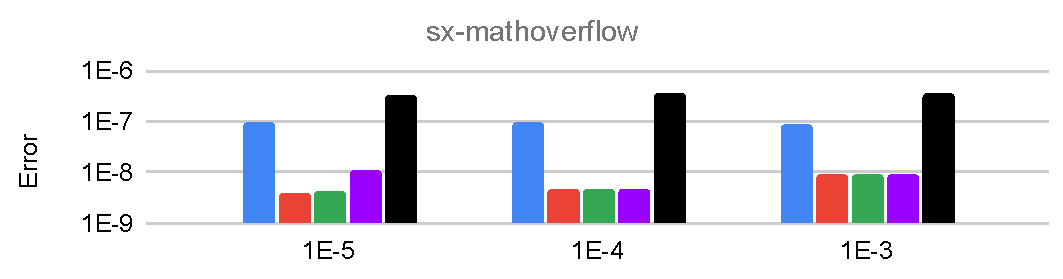
\includegraphics[width=0.48\linewidth]{out/temporal-large-error-sx-mathoverflow.pdf}
  }
  \subfigure{
    \label{fig:temporal-large--runtime}
    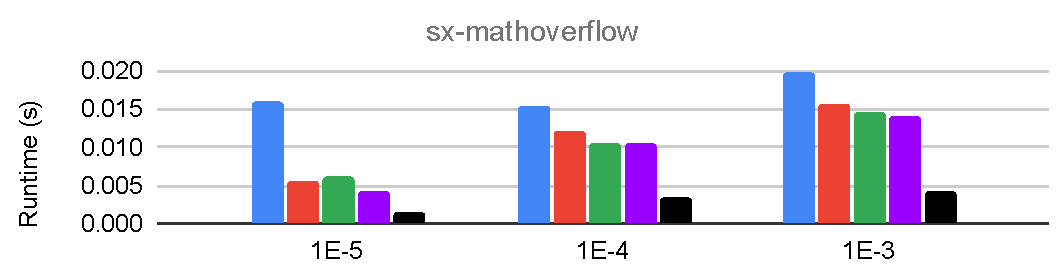
\includegraphics[width=0.48\linewidth]{out/temporal-large-runtime-sx-mathoverflow.pdf}
  }
  \subfigure{
    \label{fig:temporal-large--error}
    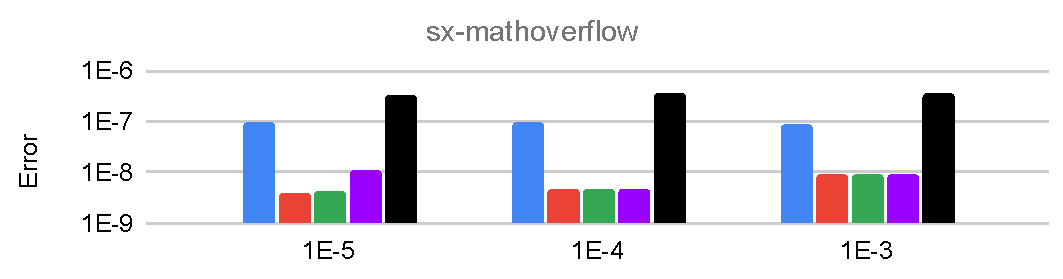
\includegraphics[width=0.48\linewidth]{out/temporal-large-error-sx-mathoverflow.pdf}
  }
  \subfigure{
    \label{fig:temporal-large--runtime}
    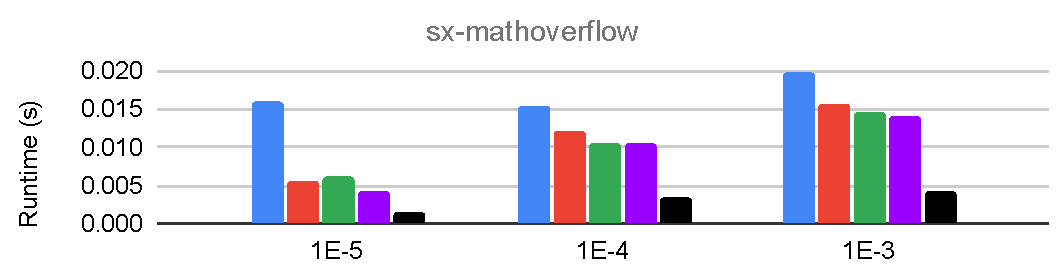
\includegraphics[width=0.48\linewidth]{out/temporal-large-runtime-sx-mathoverflow.pdf}
  }
  \subfigure{
    \label{fig:temporal-large--error}
    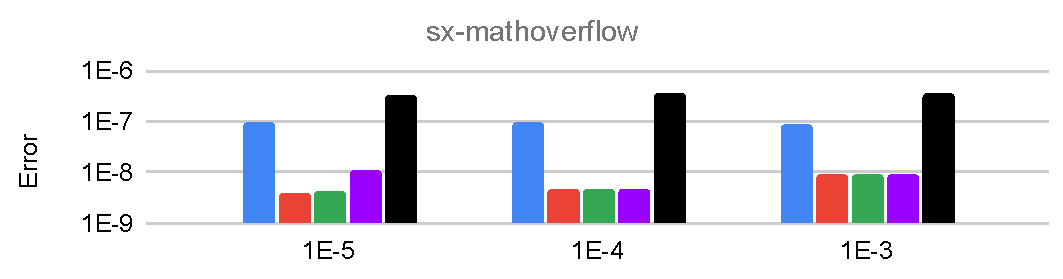
\includegraphics[width=0.48\linewidth]{out/temporal-large-error-sx-mathoverflow.pdf}
  }
  \subfigure{
    \label{fig:temporal-large--runtime}
    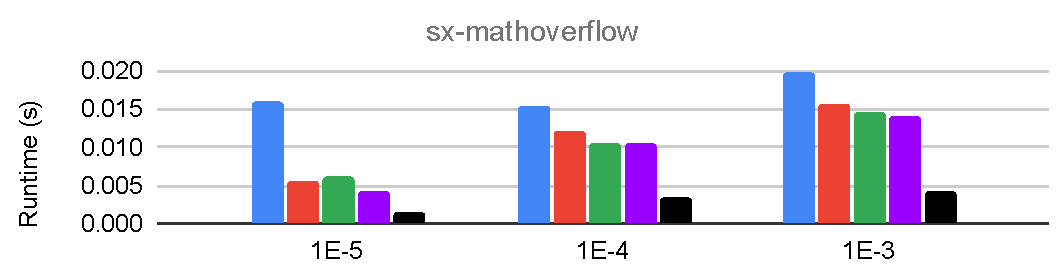
\includegraphics[width=0.48\linewidth]{out/temporal-large-runtime-sx-mathoverflow.pdf}
  }
  \subfigure{
    \label{fig:temporal-large--error}
    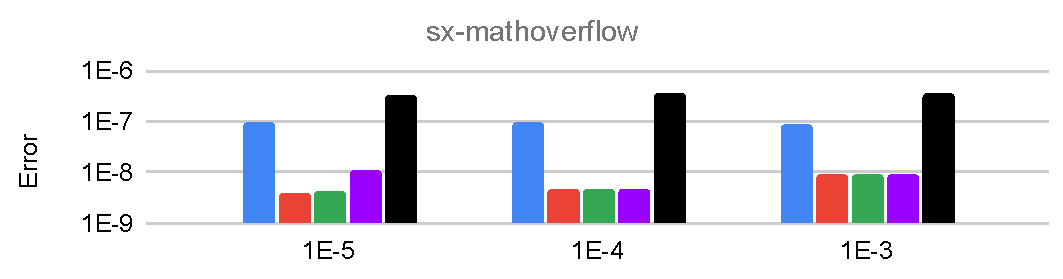
\includegraphics[width=0.48\linewidth]{out/temporal-large-error-sx-mathoverflow.pdf}
  } \\[-2ex]
  \caption{Average Relative runtime with asynchronous implementations of \textit{Static}, \textit{Naive-dynamic}, \textit{Dynamic Traversal}, and \textit{Dynamic Frontier} approach compared to their respective synchronous implementations, on batch updates of size $10^{-7}|E|$ to $0.1|E|$ (right), and overall (left). The results indicate that asynchronous implementations are faster than synchronous ones, especially for smaller batch sizes. This is due to a somewhat faster convergence and the absence of copy overhead (for \textit{Dynamic Traversal} and \textit{Dynamic Frontier} approaches).}
  \label{fig:temporal-large}
\end{figure*}

% \begin{figure*}[hbtp]
  \centering
  % \includegraphics[width=0.44\linewidth]{out/8020-runtime-key.pdf}
  \subfigure[Overall result]{
    \label{fig:8020-runtime--mean}
    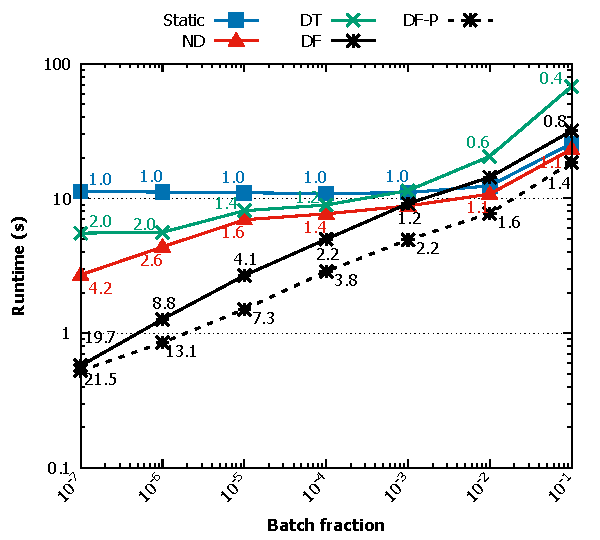
\includegraphics[width=0.38\linewidth]{out/8020-runtime-mean.pdf}
  }
  \subfigure[Results on each graph]{
    \label{fig:8020-runtime--all}
    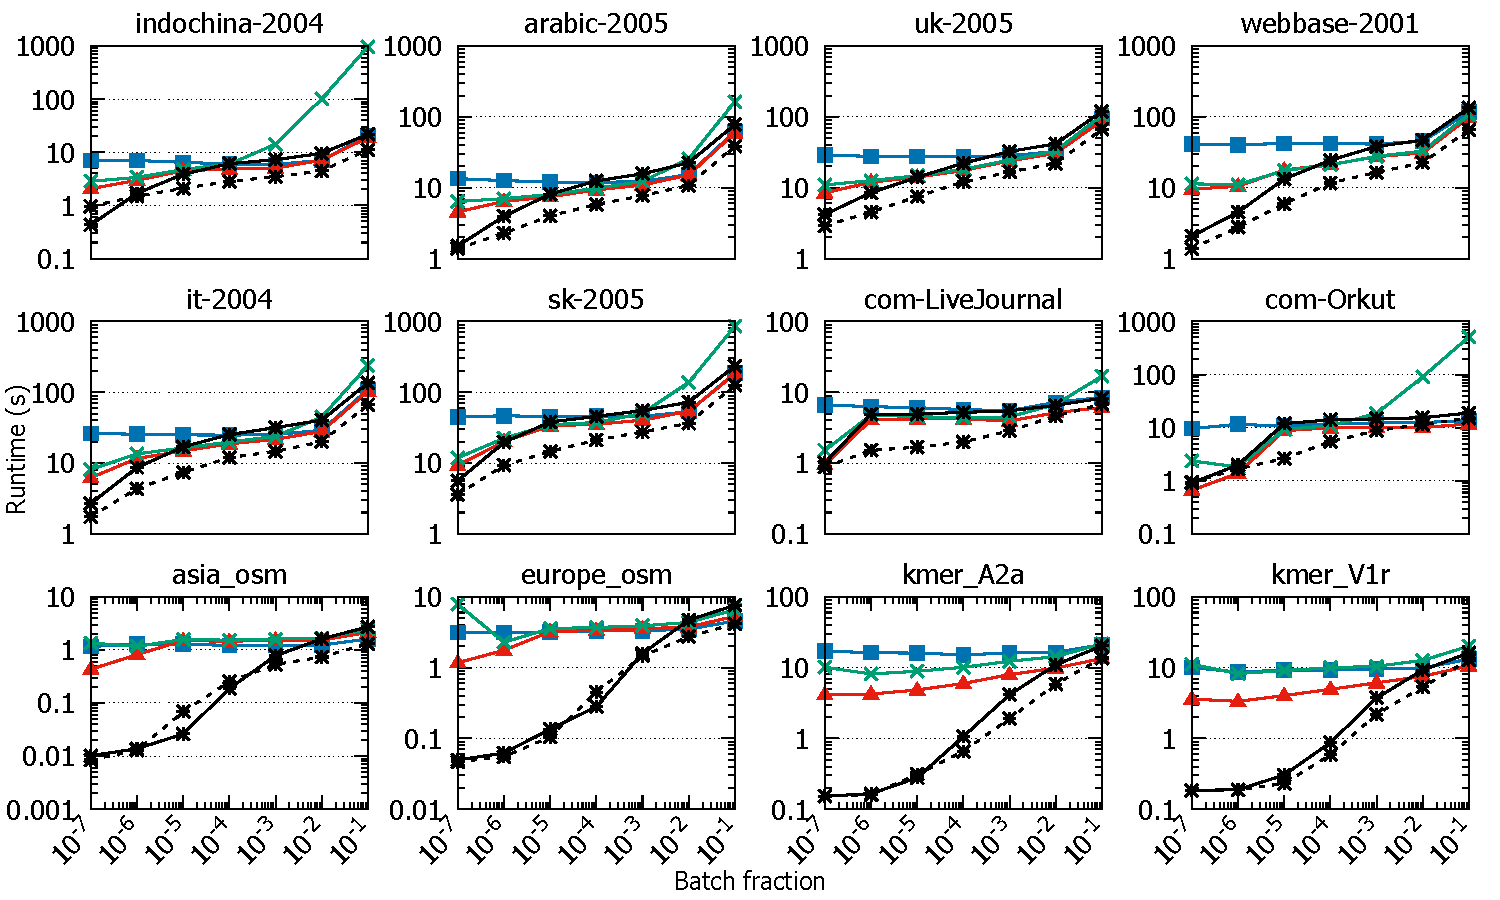
\includegraphics[width=0.58\linewidth]{out/8020-runtime-all.pdf}
  } \\[-1ex]
  \caption{Runtime (logarithmic scale) of \textit{Static}, \textit{Naive-dynamic}, \textit{Dynamic Traversal}, and \textit{Dynamic Frontier} PageRank with batch updates increasing from $10^{-7} |E|$ to $0.1 |E|$, in multiples of $10$ (logarithmic scale). The updates include $80\%$ edge insertions and $20\%$ edge deletions, simulating realistic changes upon a dynamic graph. The figure on the right illustrates the runtime of each approach for each graph in the dataset, while the figure of the left presents overall runtimes (using geometric mean for consistent scaling across graphs).}
  \label{fig:8020-runtime}
\end{figure*}

% \begin{figure*}[hbtp]
  \centering
  % \includegraphics[width=0.44\linewidth]{out/8020-speedup-key.pdf}
  \subfigure[Overall result]{
    \label{fig:8020-speedup--mean}
    \includegraphics[width=0.38\linewidth]{out/8020-speedup-mean.pdf}
  }
  \subfigure[Results on each graph]{
    \label{fig:8020-speedup--all}
    \includegraphics[width=0.58\linewidth]{out/8020-speedup-all.pdf}
  } \\[-1ex]
  \caption{Speedup of \textit{Dynamic Frontier} PageRank with respect to \textit{Static}, \textit{Naive-dynamic}, and \textit{Dynamic Traversal} PageRank on batch updates of size $10^{-7} |E|$ to $0.1 |E|$ (logarithmic scale), with $80\%$ edge insertions and $20\%$ edge deletions --- representing a realistic batch update upon a dynamic graph. The figure on the right shows the speedup of \textit{Dynamic Frontier} PageRank, with respect to each approach, for each graph in the dataset --- while the figure of the left highlights the overall speedup.}
  \label{fig:8020-speedup}
\end{figure*}

% \begin{figure*}[hbtp]
  \centering
  \subfigure[Overall result]{
    \label{fig:8020-error--mean}
    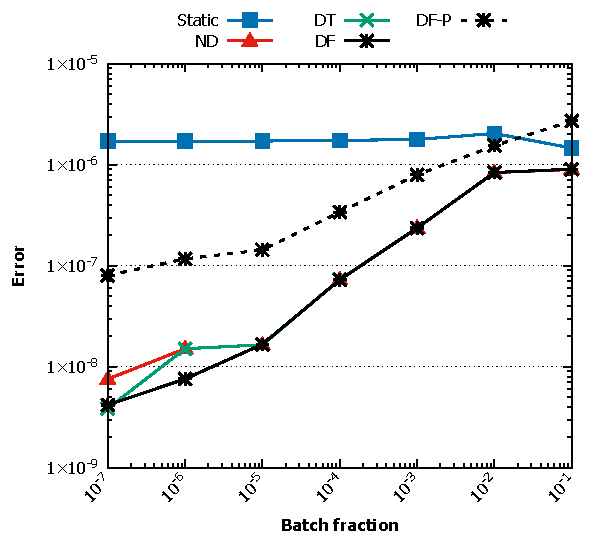
\includegraphics[width=0.38\linewidth]{out/8020-error-mean.pdf}
  }
  \subfigure[Results on each graph]{
    \label{fig:8020-error--all}
    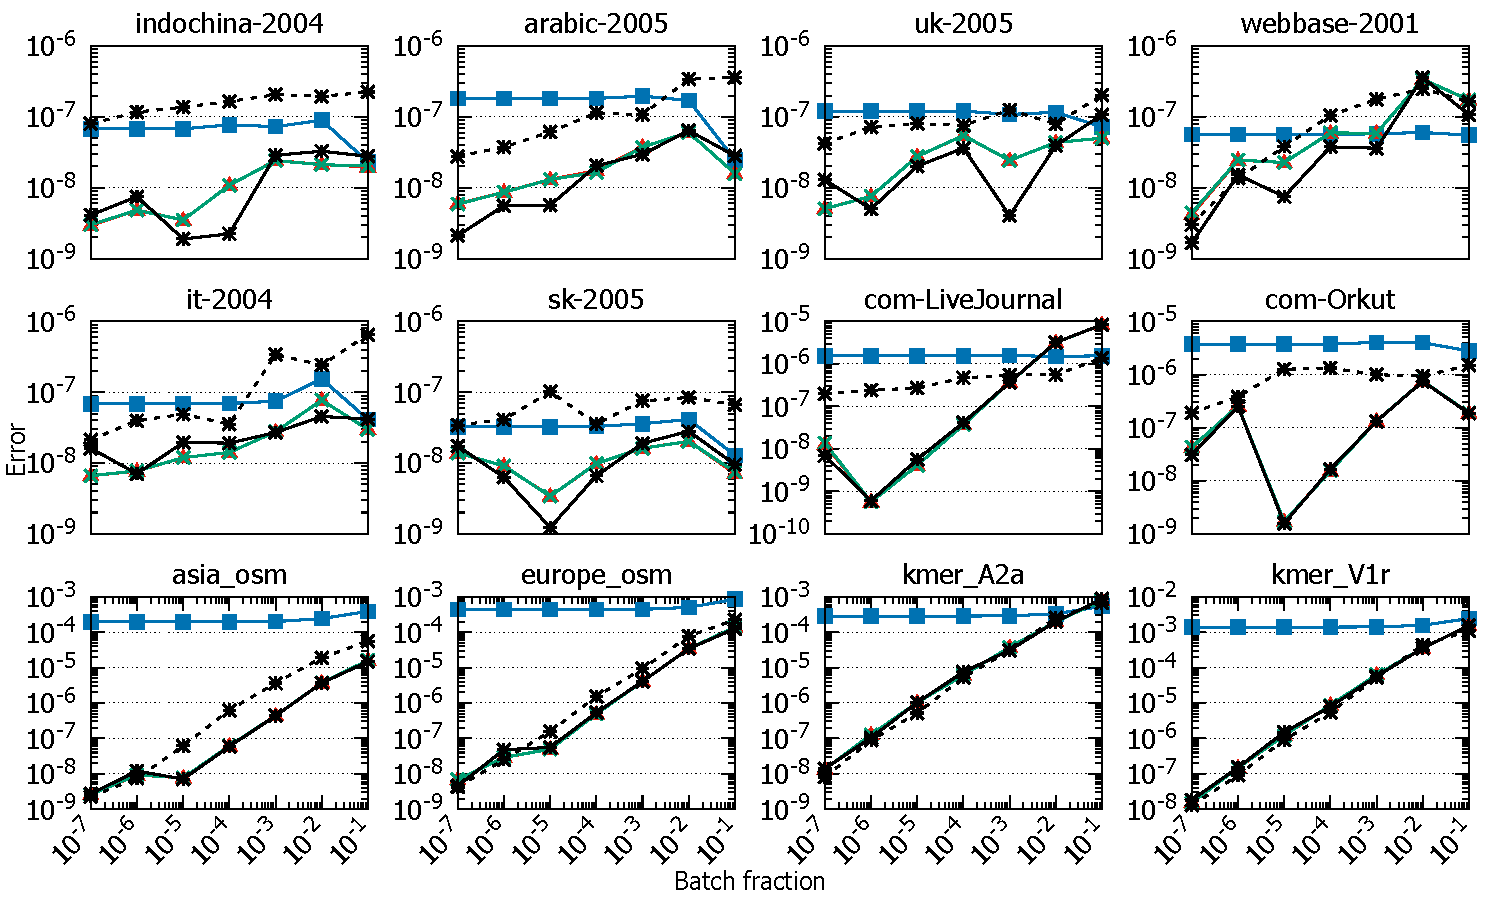
\includegraphics[width=0.58\linewidth]{out/8020-error-all.pdf}
  } \\[-1ex]
  \caption{Error comparison of \textit{Static}, \textit{Naive-dynamic (ND)}, \textit{Dynamic Traversal (DT)}, our improved \textit{Dynamic Frontier (DF)}, and \textit{Dynamic Frontier with Pruning (DF-P)} PageRank on large (static) graphs with generated random batch updates, relative to a Reference Static PageRank (see Section \ref{sec:measurement}), using $L1$-norm. The size of batch updates range from $10^{-7} |E|$ to $0.1 |E|$ in multiples of $10$ (logarithmic scale), consisting of $80\%$ edge insertions and $20\%$ edge deletions to simulate realistic dynamic graph updates. The right subfigure depicts the error for each approach in relation to each graph, while the left subfigure showcases overall errors using geometric mean for consistent scaling across graphs.}
  \label{fig:8020-error}
\end{figure*}

% \begin{figure}[!hbt]
  \centering
  \subfigure{
    \label{fig:measure-affected--batch}
    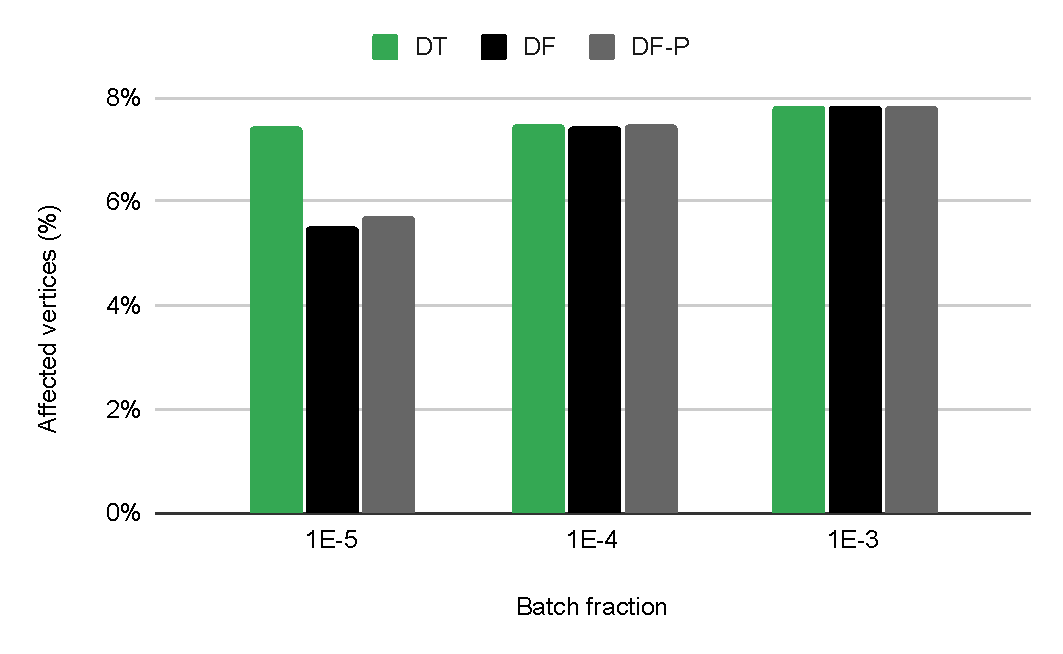
\includegraphics[width=0.98\linewidth]{out/measure-affected-batch.pdf}
  } \\[-2ex]
\caption{Average percentage of vertices marked as affected by \textit{Dynamic Traversal} and \textit{Dynamic Frontier} PageRank, with batch size increasing from $10^{-7} |E|$ to $0.1 |E|$ in multiples of $10$ (logarithmic scale), consisting purely of edge insertions. The \textit{Dynamic Frontier} approach marks affected vertices incrementally --- thus, the final percentage (at the end of all iterations) is depicted here.}
  \label{fig:measure-affected}
\end{figure}





\subsection{Performance of Dynamic Frontier PageRank}

We first study the performance of Dynamic Frontier PageRank on batch updates of size $10^{-7}|E|$ to $0.1|E|$ (in multiples of $10$), consisting purely of edge insertions, and compare it with Static, Naive-dynamic, and Dynamic Traversal PageRank. As mentioned above, the edge insertions are generated uniformly at random. Figure \ref{fig:insertions-runtime} plots the runtime of Static, Naive-dynamic, Dynamic Traversal, and Dynamic Frontier PageRank; Figure \ref{fig:insertions-speedup} plots the speedup of Dynamic Frontier PageRank with respect to Static, Naive-dynamic, and Dynamic Traversal PageRank; and Figure \ref{fig:insertions-error} plots the error in ranks obtained with Static, Naive-dynamic, Dynamic Traversal, and Dynamic Frontier PageRank with respect to ranks obtained from a reference Static PageRank (see Section \ref{sec:measurement}). In a similar manner, Figures \ref{fig:deletions-runtime}, \ref{fig:deletions-speedup}, and \ref{fig:deletions-error} present the runtime, speedup, and rank errors of each approach on batch updates consisting purely of edge deletions. Finally, Figures \ref{fig:8020-runtime}, \ref{fig:8020-speedup}, and \ref{fig:8020-error} present the runtime, speedup, and error with each approach on batch updates consisting of an $80\%$ / $20\%$ mix of edge insertions and deletions, in order to simulate realistic batch updates.


\subsubsection{Results with insertions-only batch updates}

Dynamic Frontier PageRank is on average $8.3\times$, $2.7\times$, and $3.4\times$ faster than Static, Naive-dynamic, and Dynamic Traversal PageRank on insertions-only batch updates of size $10^{-7}|E|$ to $10^{-3}|E|$, while obtaining ranks of better accuracy/error than Static PageRank, and of similar accuracy/error as Naive-dynamic and Dynamic Traversal PageRank. On road networks, and protein k-mer graphs, Dynamic Frontier PageRank is significantly faster than its competitors (Naive-dynamic and Dynamic Traversal PageRank).


\subsubsection{Results with deletions-only batch updates}

On deletions-only batch updates of size $10^{-7}|E|$ to $10^{-3}|E|$, Dynamic Frontier PageRank is on average $7.4\times$, $3.1\times$, and $4.1\times$ faster than Static, Naive-dynamic, and Dynamic Traversal PageRank, while obtaining ranks of better accuracy/error than Static PageRank (for batch sizes less than $0.1|E|$), and of similar accuracy/error as Naive-dynamic and Dynamic Traversal PageRank. On \textit{indochina-2004}, \textit{webbase-2001}, road networks, and protein k-mer graphs, Dynamic Frontier PageRank is significantly faster than its competitors (Naive-dynamic and Dynamic Traversal PageRank).


\subsubsection{Results with 80\%-20\% mix batch updates}

On batch updates of size $10^{-7}|E|$ to $10^{-3}|E|$, consisting of $80\%$ insertions and $20\%$ deletions, Dynamic Frontier PageRank is on average $7.6\times$, $2.8\times$, and $4.1\times$ faster than Static, Naive-dynamic, and Dynamic Traversal PageRank, while obtaining ranks of better accuracy/error than Static PageRank, and of similar accuracy/error as Naive-dynamic and Dynamic Traversal PageRank. Similar to deletions-only batch updates, Dynamic Frontier PageRank outperforms its competitors (Naive-dynamic and Dynamic Traversal PageRank) on \textit{indochina-2004}, \textit{webbase-2001}, road networks, and protein k-mer graphs.
% This seems to be associated to sparsity of the graphs as Dynamic Frontier PageRank performing well on sparse graphs.


\subsubsection{Results with temporal graphs}

We also attempt Static, Naive-dynamic, Dynamic Traversal, and Dynamic Frontier PageRank on temporal graphs found in the Stanford Large Network Dataset Collection \cite{snap14}. On some temporal graphs, Dynamic Frontier PageRank does not outperform its competitors with a frontier tolerance of $\tau_f = \tau / 10^5$, where $\tau$ is the iteration tolerance. However, choosing a lower $\tau_f$ of $\tau / 10$ or $\tau / 100$ allows it achieve good performance. Thus, the choice of frontier tolerance $\tau_f$, possibly in addition to how the frontier of affected vertices is expanded, is dependent upon the nature of the batch update. We plan to explore this in the future.


\subsubsection{Comparison of vertices marked as affected}

Figure \ref{fig:measure-affected} shows the total number of vertices marked as affected (average) by Dynamic Traversal and Dynamic Frontier PageRank on batch updates of size $10^{-7}|E|$ to $0.1|E|$, consisting exclusively of edge insertions. The Dynamic Frontier approach marks affected vertices incrementally --- thus, the final percentage (at the end of all iterations) is depicted in the figure. It is observed that Dynamic Traversal PageRank marks a higher percentage of vertices as affected, even for small batch updates.\ignore{This is likely due the randomly generated edges in the batch update being part of large Strongly Connected Components (SCCs), or due to a large number of such SCCs being reachable from the vertices that are part of the batch update.} In contrast, Dynamic Frontier PageRank marks far fewer vertices as affected, as it incrementally expands the affected region of the graph only after the rank of an affected vertex changes by a substantial amount, i.e., by frontier tolerance $\tau_f = \tau / 10^5$, where $\tau$ is the iteration tolerance (using $L\infty$-norm). In addition, as Dynamic Frontier PageRank incrementally marks vertices as affected, the actual work performed by the algorithm is lower than that indicated by the percentage of affected vertices in Figure \ref{fig:measure-affected}.

\begin{figure}[!hbt]
  \centering
  \subfigure{
    \label{fig:strong-scaling--speedup}
    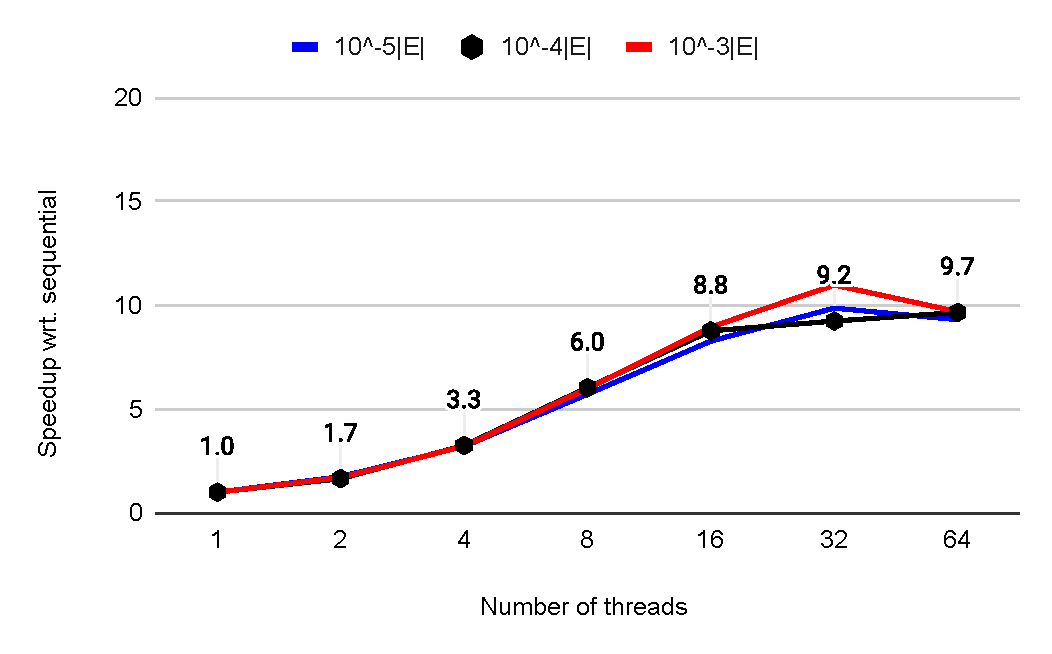
\includegraphics[width=0.98\linewidth]{out/strong-scaling-speedup.pdf}
  } \\[-2ex]
  \caption{Mean speedup of \textit{Dynamic Frontier (DF)} PageRank with increasing number of threads (in multiples of $2$), on real world dynamic graphs, with batch sizes of $10^{-5}|E|$ to $10^{-3}|E|$\ignore{ (consisting purely of edge insertions)}.}
  \label{fig:strong-scaling}
\end{figure}
%% TODO: Update this





\subsection{Strong Scaling of Dynamic Frontier PageRank}

Finally, we study the strong-scaling behavior of Dynamic Frontier PageRank on batch updates of a fixed size of $10^{-4} |E|$, consisting purely of edge insertions. Here, we measure the speedup of Dynamic Frontier PageRank with an increasing number of threads from $1$ to $64$ in multiples of $2$ with respect to a single-threaded execution of the algorithm. This is repeated for each graph in the dataset, and the results are averaged (using geometric mean).

The results are shown in Figure \ref{fig:strong-scaling}. With $16$ threads, Dynamic Frontier PageRank achieves an average speedup of $10.3\times$, compared to a single-threaded execution, indicating a performance increase of $1.8\times$ for every doubling of threads. At $32$ and $64$ threads, Dynamic Frontier PageRank is affected by NUMA effects (the $64$-core processor we use has $4$ NUMA domains), resulting in a speedup of only $14.3\times$ and $15.2\times$ respectively.

\ignore{\begin{figure}[!hbt]
  \centering
  \subfigure{
    \label{fig:weak-scaling--speedup}
    \includegraphics[width=0.98\linewidth]{out/weak-scaling-speedup.pdf}
  } \\[-2ex]
  \caption{Average speedup of \textit{Dynamic Frontier} PageRank with increasing number of threads (in multiples of $2$), on a batch sizes of $10^{-4}|E|$ to $6.4\times10^{-3}|E|$ (consisting purely of edge insertions), increasing in multiples of $2$ in tandem with the increase in the number of threads.}
  \label{fig:weak-scaling}
\end{figure}
}
